\documentclass{article}
\usepackage{graphicx} %package to manage images
\usepackage[utf8]{inputenc}
\usepackage[a4paper, total={6in, 8in}]{geometry}
\usepackage{xurl}
\usepackage{hyperref}
\usepackage{float}
\title{Relatório 6 \\ Matching}
\author{Pedro A. S. O. Neto}
\date{Junho, 2023}

\begin{document}

\maketitle

\section{Matching between samples}

There were notable discrepancies in age between our original samples of TD and TEA participants (Table 1). Additionally, there was a significant gender(?) imbalance, with x\% of females in the TD group, and only x\% in amongst TEA participants (see table 1).

\begin{table}[ht]
\caption(Age distribution, in months, between sex and tea participants)
\centering
\begin{tabular}{rllrrr}
  \hline
 & sexo & tea & sdAgeJA & meanAgeJA & N \\ 
  \hline
1 & F & TD & 1.00 & 2.89 & 188 \\ 
  2 & F & TEA &  & 2.00 &   1 \\ 
  3 & F & nonTD & 0.83 & 3.03 &   5 \\ 
  4 & F & other & 1.59 & 2.54 &   2 \\ 
  5 & F &  & 1.06 & 3.38 &   4 \\ 
  6 & M & TD & 1.04 & 2.78 & 203 \\ 
  7 & M & TEA & 0.84 & 2.93 &  22 \\ 
  8 & M & nonTD & 0.69 & 3.48 &   8 \\ 
  9 & M & other & 0.74 & 3.15 &   4 \\ 
  10 & M &  & 0.83 & 3.05 &   7 \\ 
  11 & nan &  &  &  &   3 \\ 
   \hline
\end{tabular}
\end{table}

To address this issue, we employed a matching algorithm suggested by Ho, Imai, King \& Stuart (2011), which minimized the Euclidean distance based on participants' sex and age. Following the matching process, our final sample consisted of 15 participants from each diagnostic group (refer to Table 2 and 3 for descriptive statistics before and after matching algorithm).

\begin{table}[ht]
\caption{Non matched}
\centering
\begin{tabular}{rlrrrrr}
  \hline
 & tea & meanAge & sdAge & N & minAge & maxAge \\ 
  \hline
1 & TD & 0.09 & 0.03 & 378 &   6 &  55 \\ 
  2 & TEA & 0.09 & 0.03 &  23 &  13 &  56 \\ 
   \hline
\end{tabular}
\end{table}

\begin{table}[ht]
\caption{Matched}
\centering
\begin{tabular}{rllrrrrr}
  \hline
 & tea & sexo & meanAge & sdAge & N & minAge & maxAge \\ 
  \hline
1 & TD & F & 2.00 &  &   1 & 2.00 & 2.00 \\ 
  2 & TD & M & 2.86 & 0.84 &  22 & 1.08 & 4.58 \\ 
  3 & TEA & F & 2.00 &  &   1 & 2.00 & 2.00 \\ 
  4 & TEA & M & 2.88 & 0.85 &  22 & 1.08 & 4.67 \\ 
   \hline
\end{tabular}
\end{table}



\begin{table}[H]
\caption{Matched}
\centering
\begin{tabular}{rllrrrr}
  \hline
  & tea & sexo & meanAge & sdAge & minAge & maxAge \\ 
  \hline
  1 & TD & F & 2.08 &  & 2.08 & 2.08 \\ 
  2 & TD & M & 3.13 & 0.77 & 2.21 & 4.66 \\ 
  3 & TEA & F & 2.08 &  & 2.08 & 2.08 \\ 
  4 & TEA & M & 3.13 & 0.77 & 2.21 & 4.70 \\ 
   \hline
\end{tabular}
\end{table}

\section{ANOVA}

Mixed designs anova with diagnostic (TEA vs TD) as between subjects factor, condition (IJA vs RJA), AOI pair (alternancias), AOI (Proportion fixations) as within subjects factor.

\subsection{Alternancias}

\begin{figure}[H]
  \caption{ANOVA table for alternancias}
  \noindent\makebox[\textwidth]{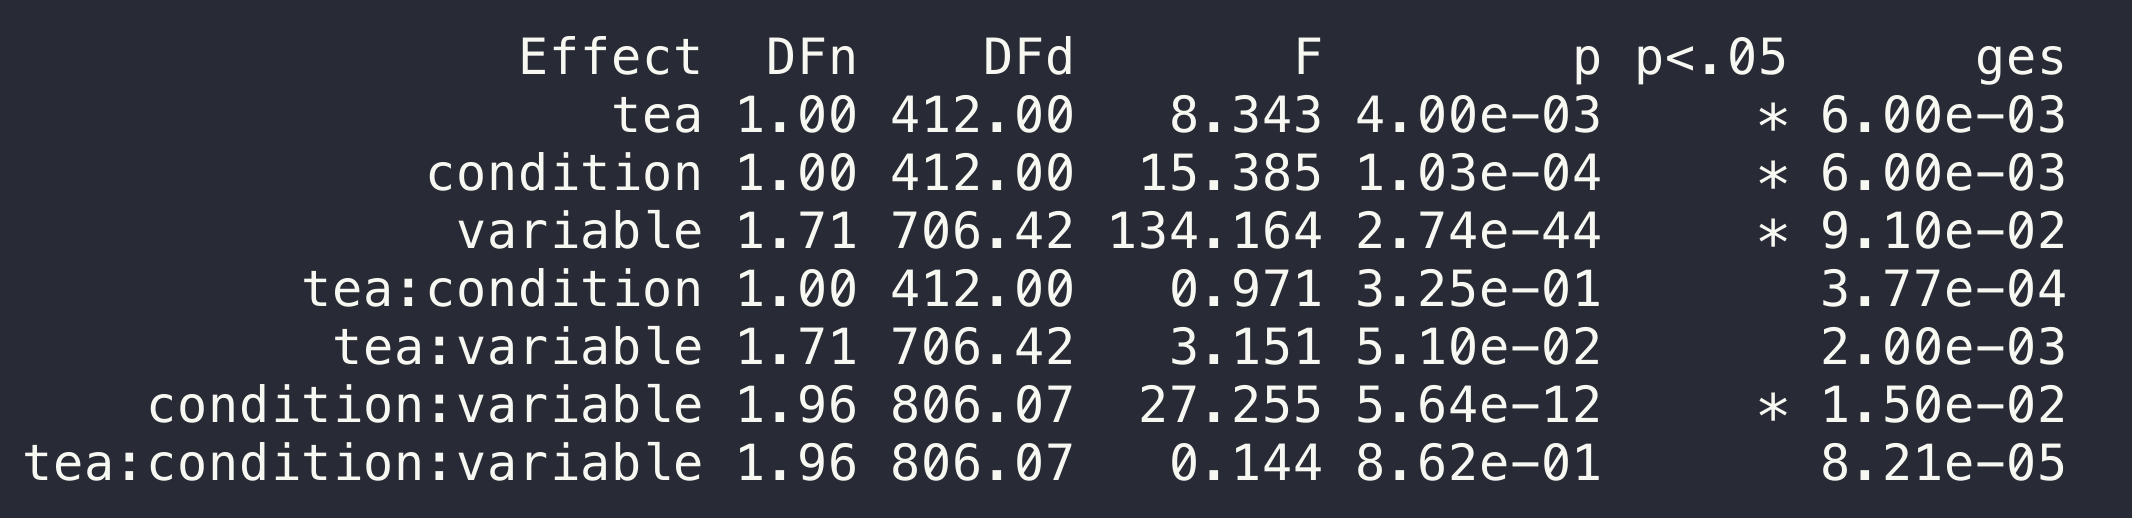
\includegraphics[scale=0.5]{./anovaAlternancia.png}}
  \centering
\end{figure}

\begin{figure}[H]
  \caption{Main effect tea}
  \noindent\makebox[\textwidth]{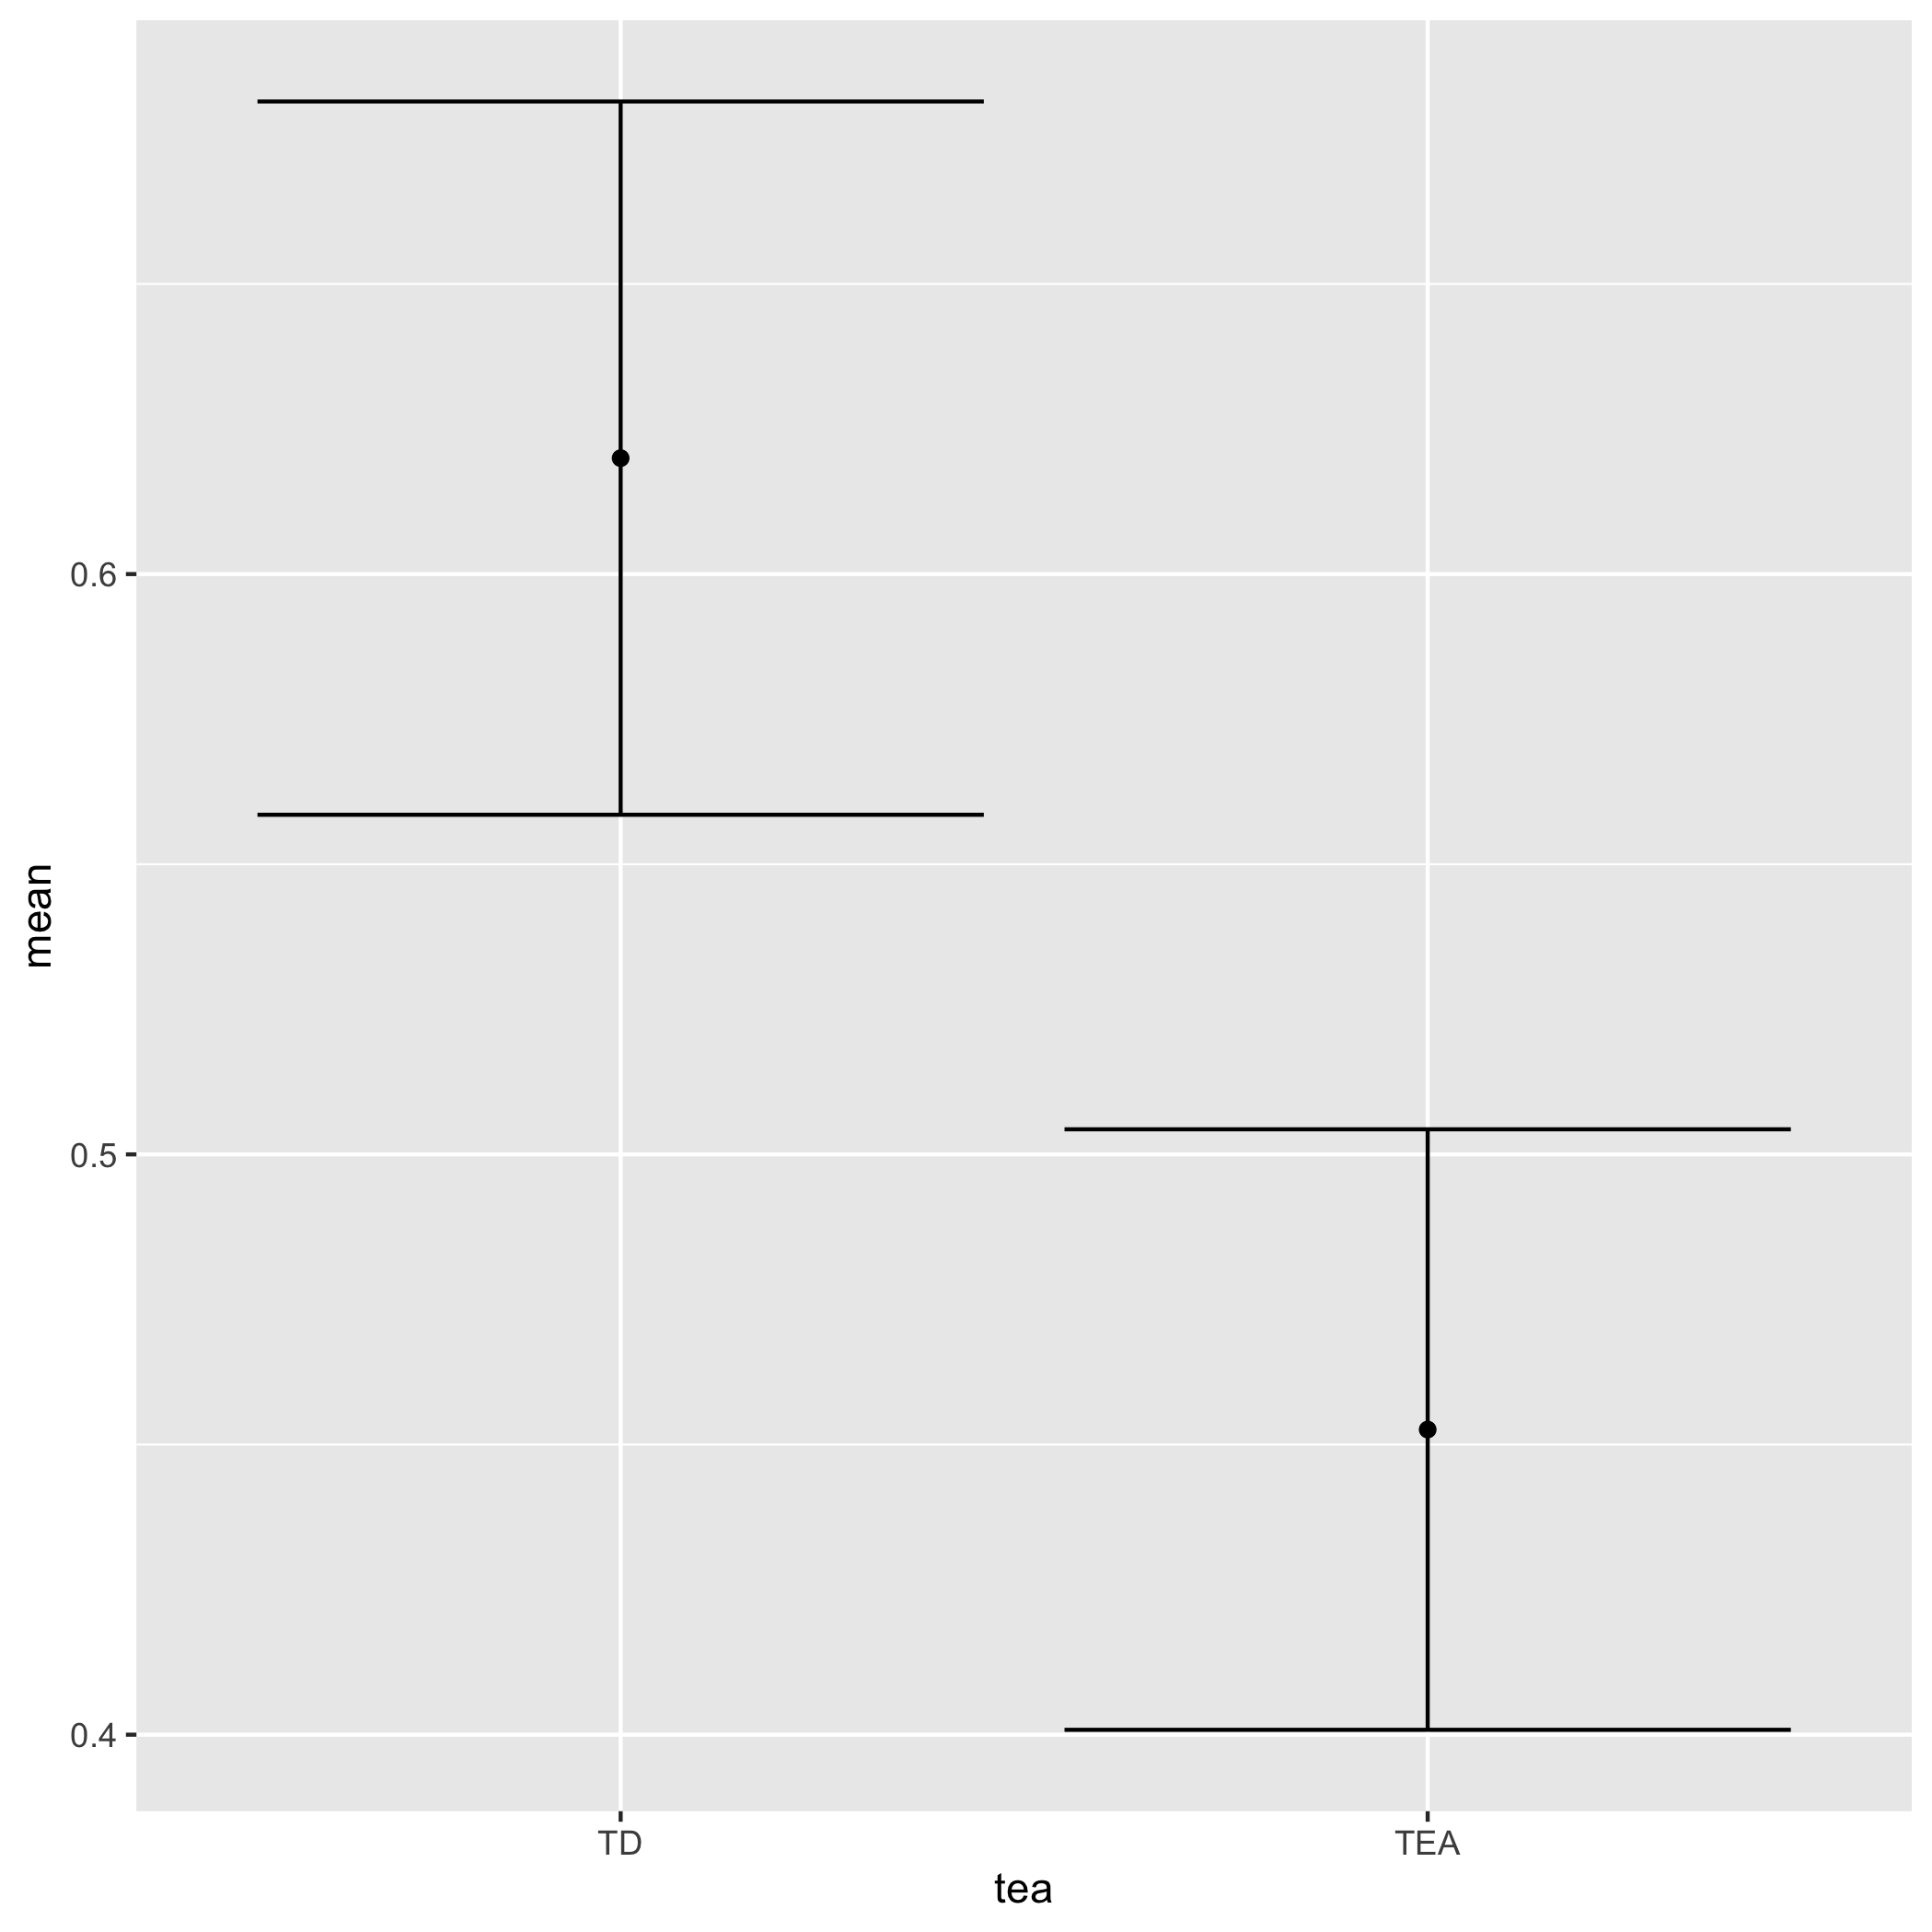
\includegraphics[scale=0.2]{./teaMainAlternancia.png}}
  \centering
\end{figure}

\begin{figure}[H]
  \caption{Visualizing effect of variable}
  \noindent\makebox[\textwidth]{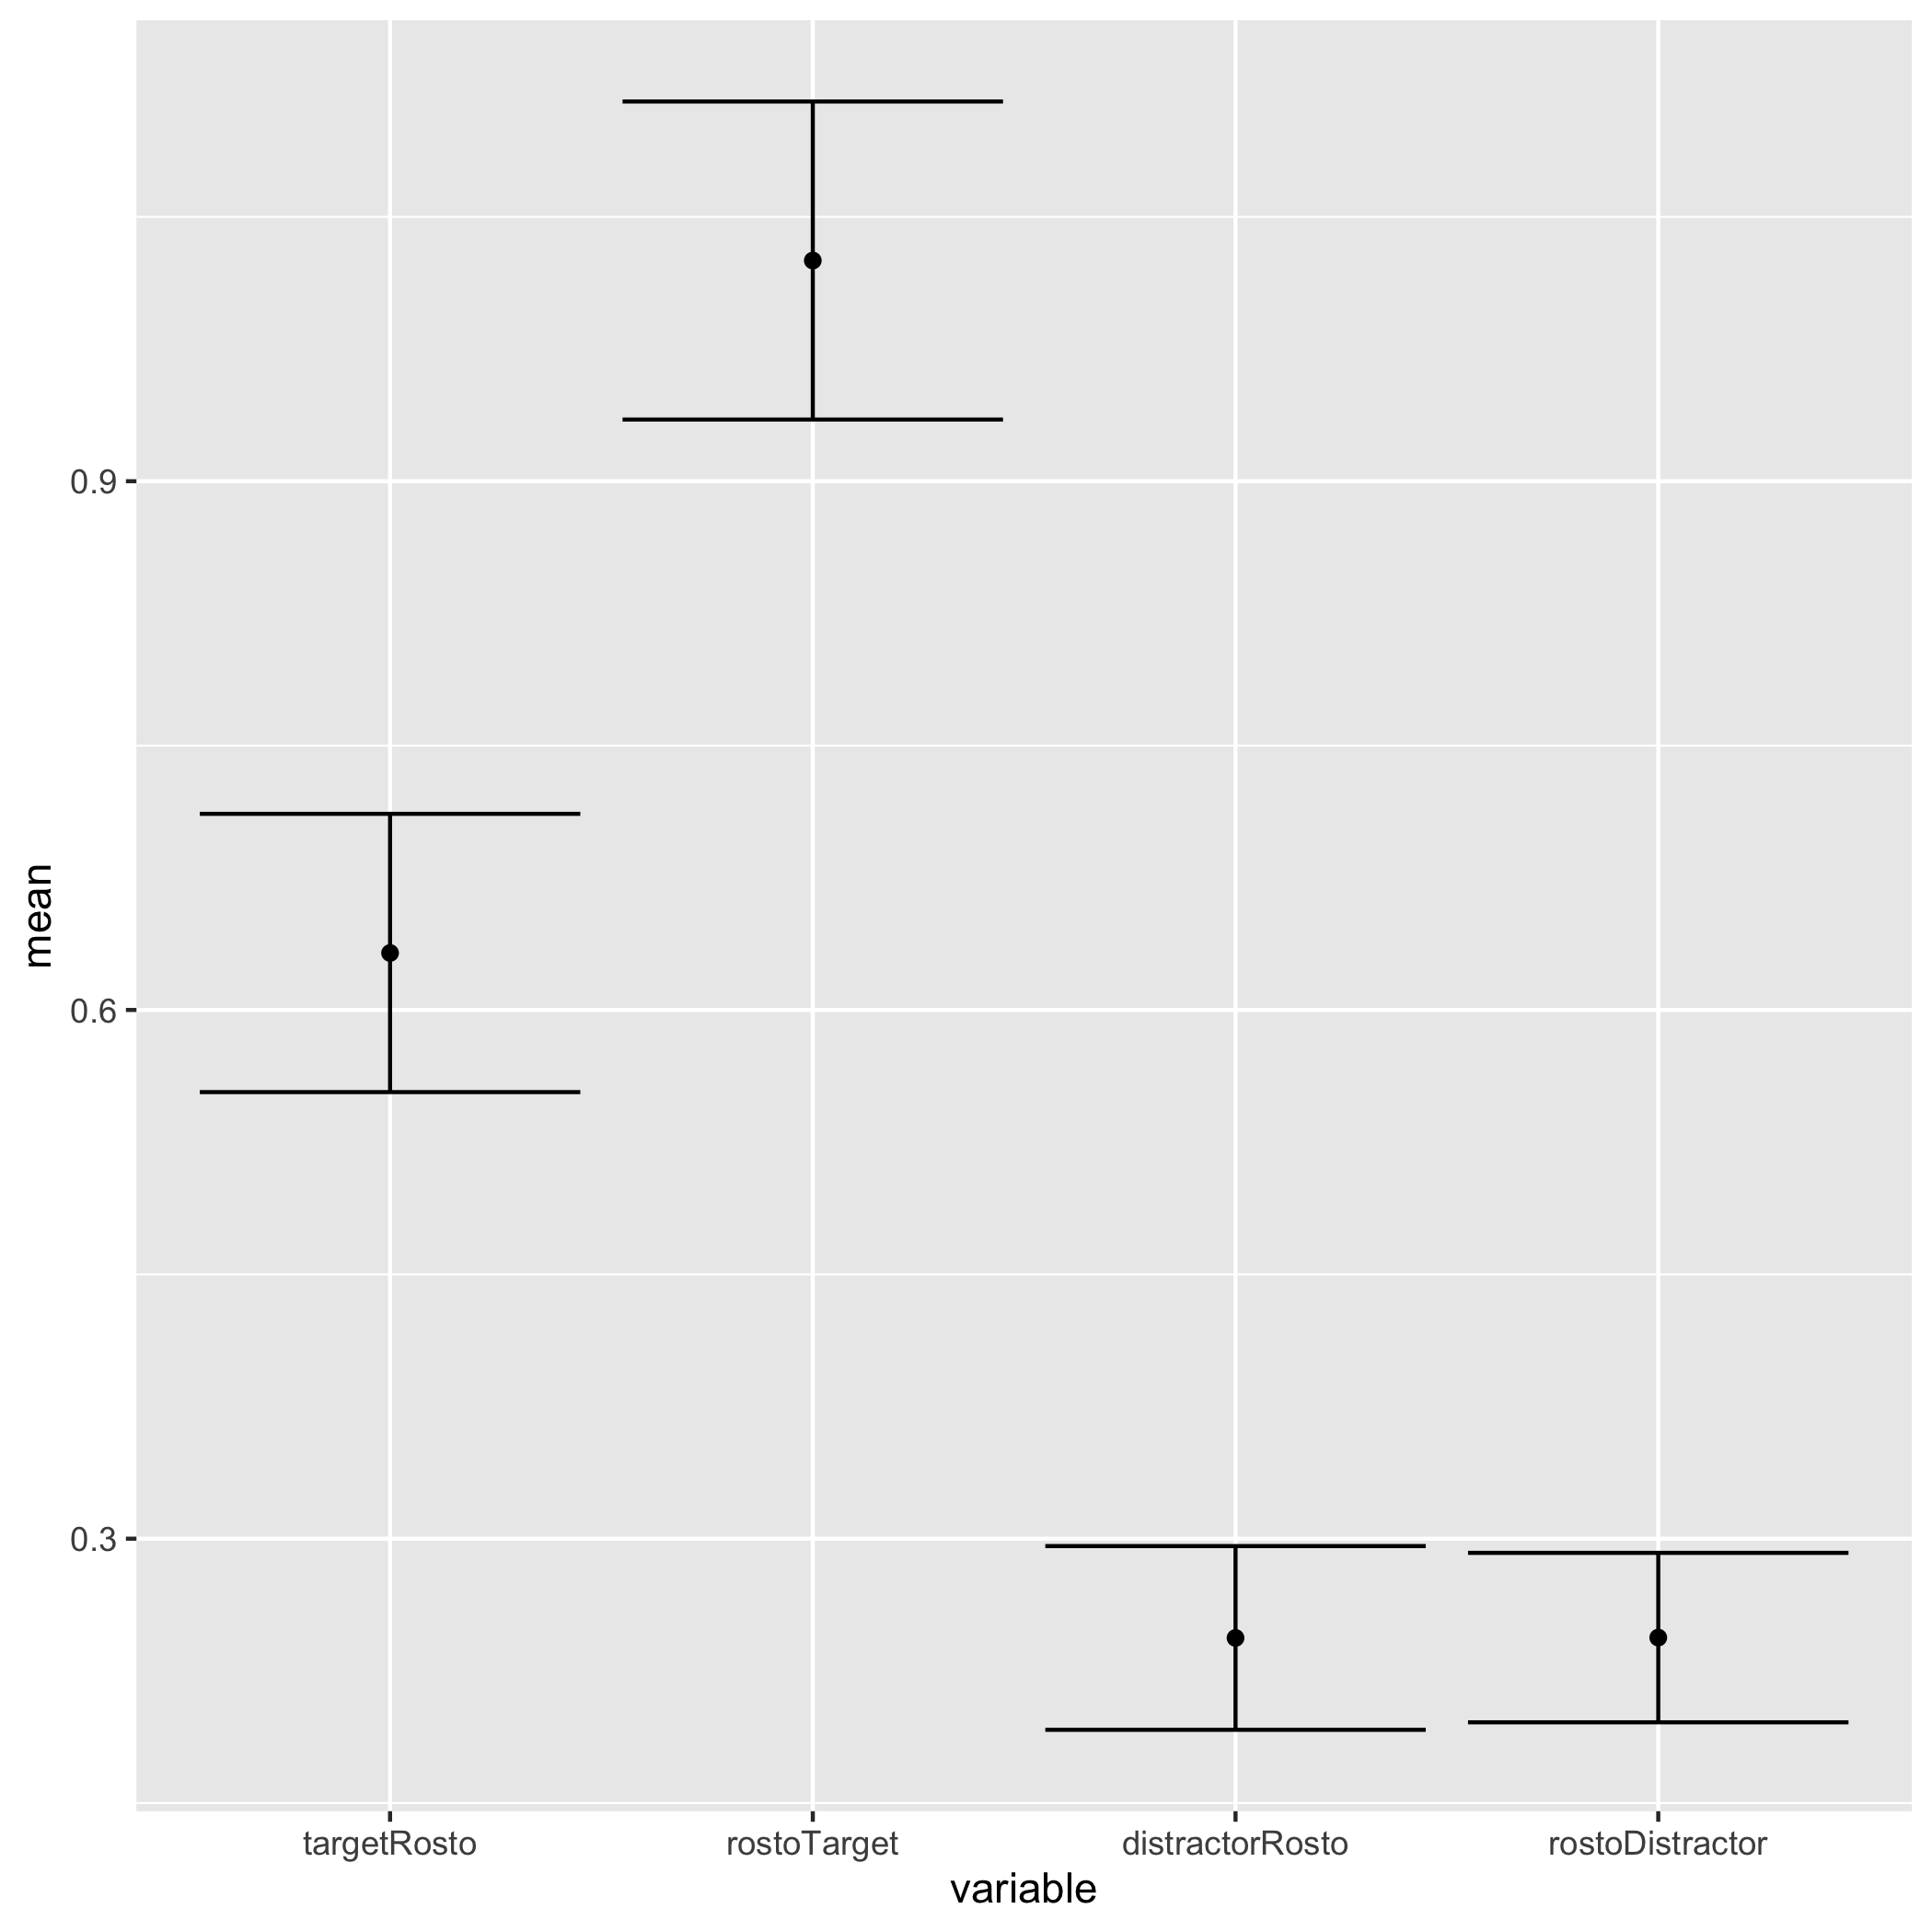
\includegraphics[scale=0.2]{./variableAlternancia.png}}
  \centering
\end{figure}

\begin{figure}[H]
  \caption{Visualizing effect of condition}
  \noindent\makebox[\textwidth]{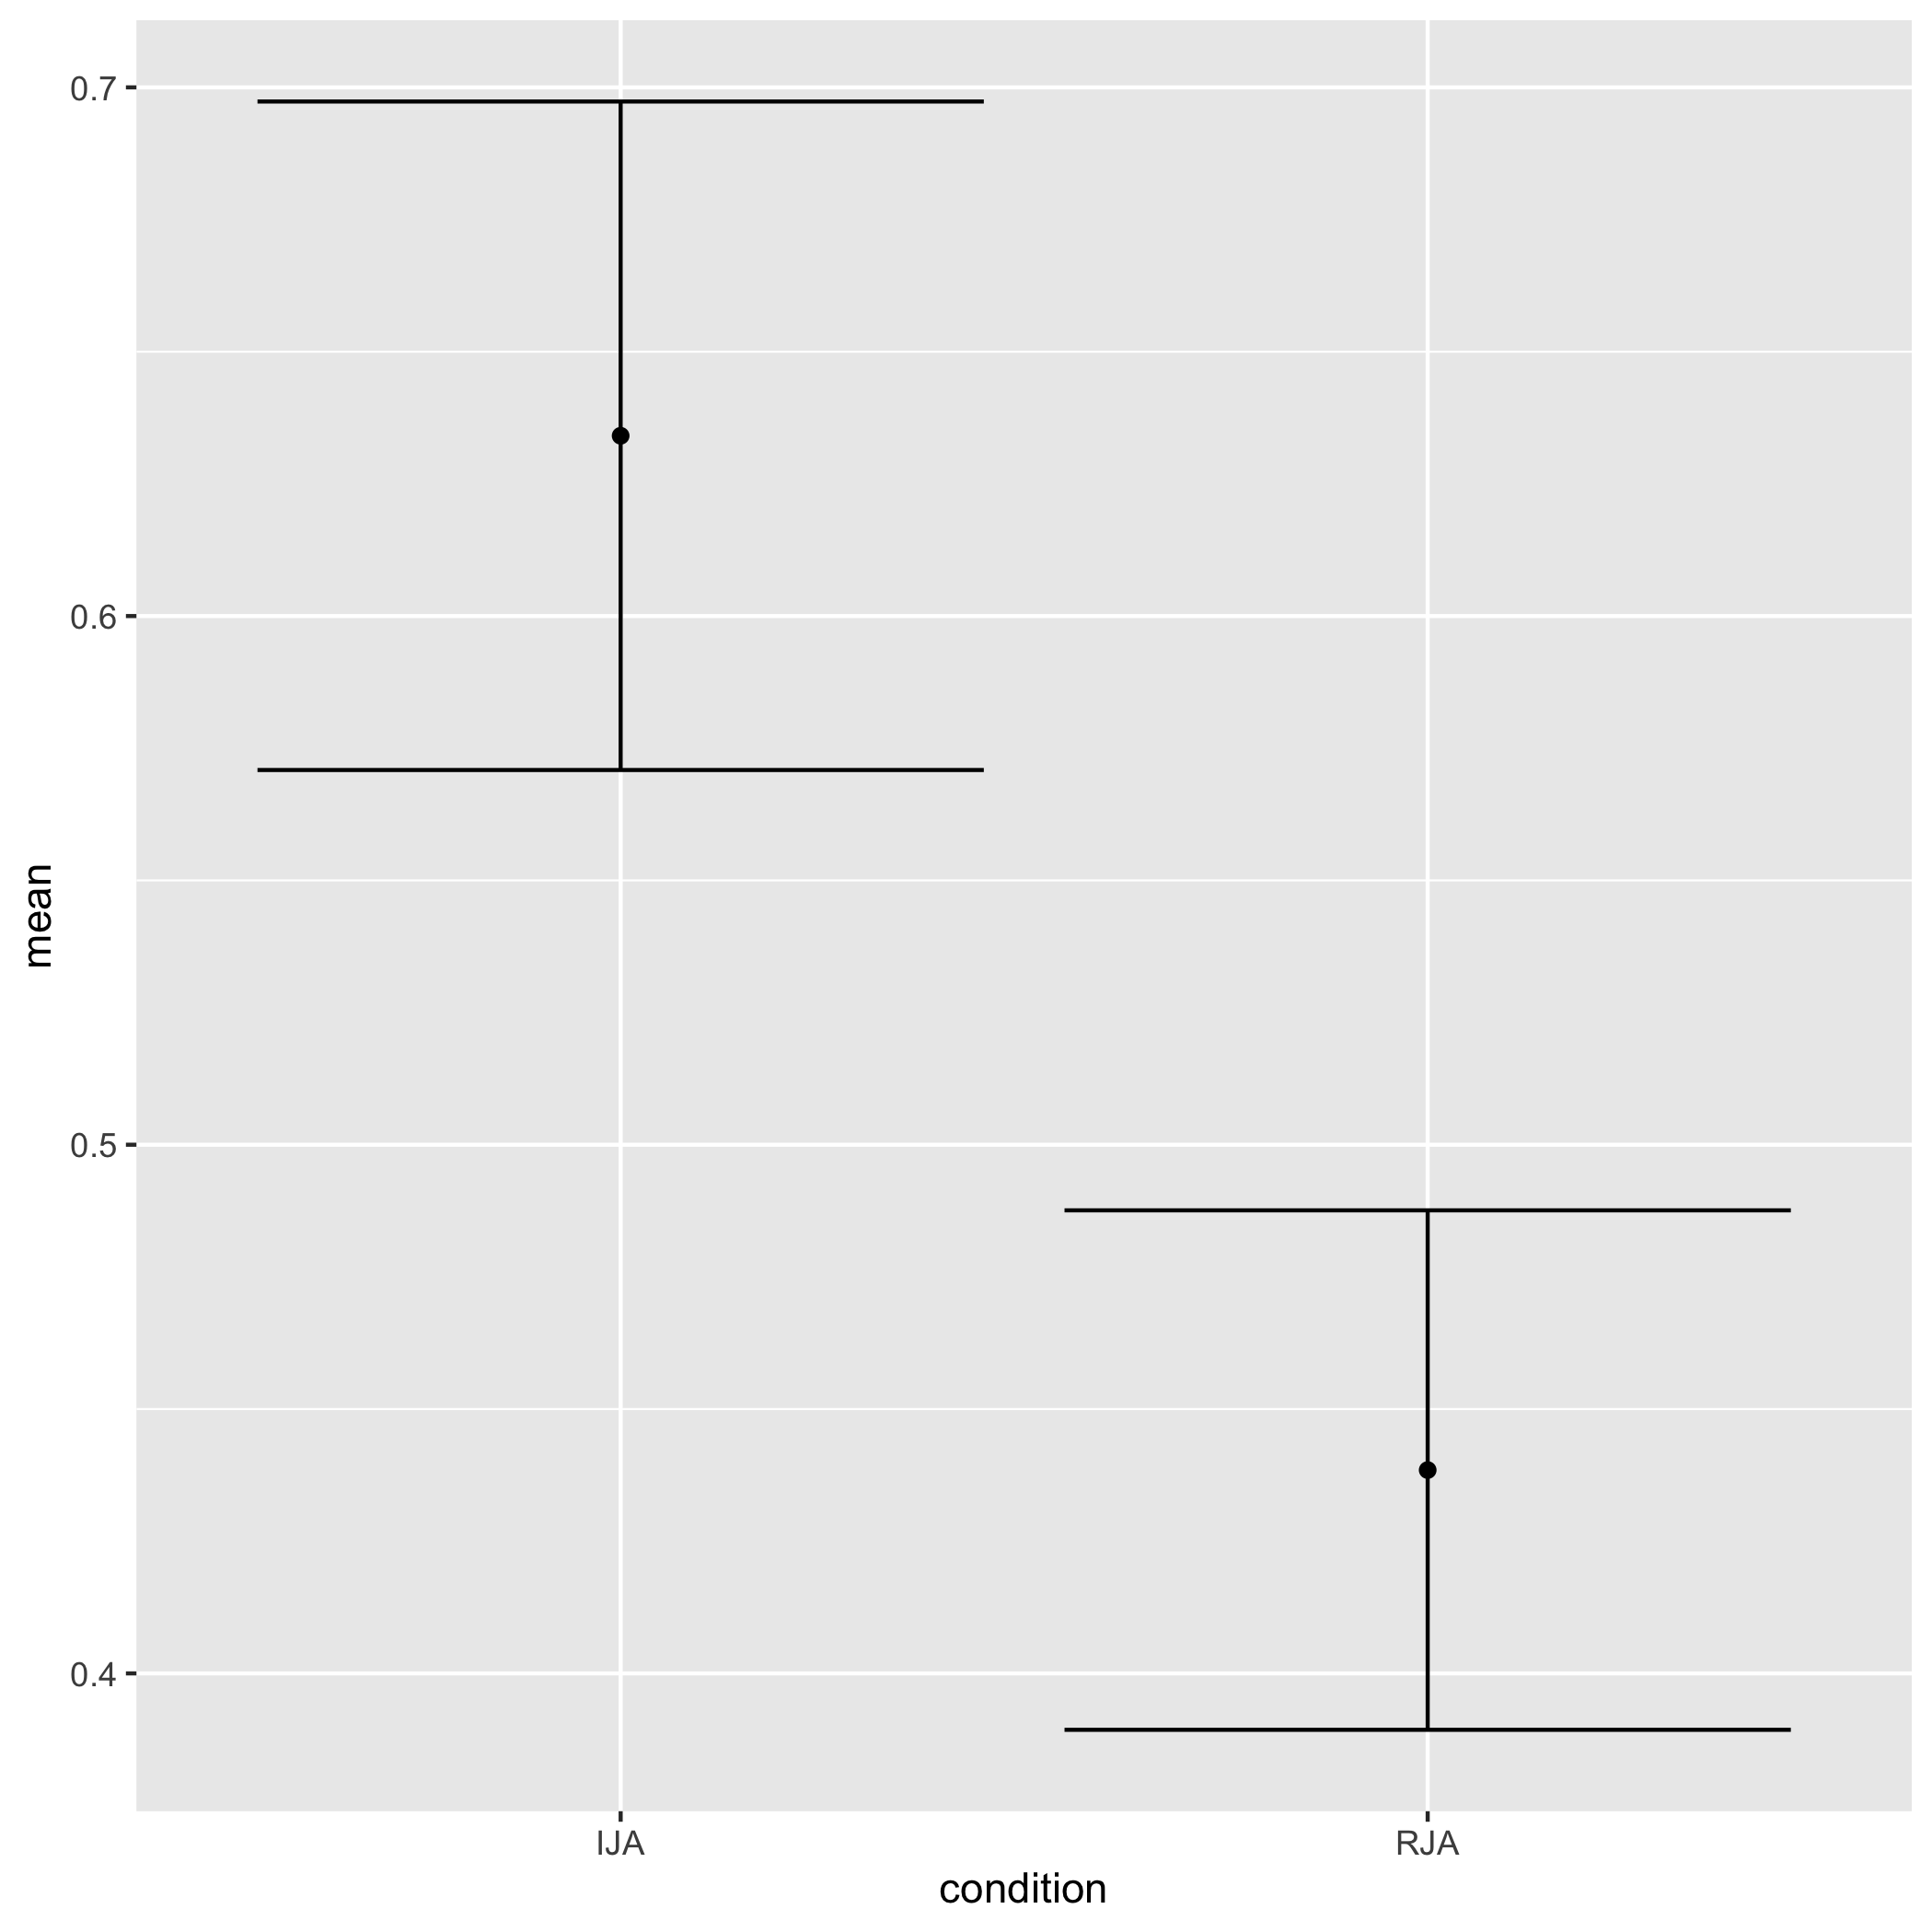
\includegraphics[scale=0.2]{./conditionAlternancia.png}}
  \centering
\end{figure}

\begin{figure}[H]
  \caption{Visualizing interaction of condition, variable and tea. *non significant}
  \noindent\makebox[\textwidth]{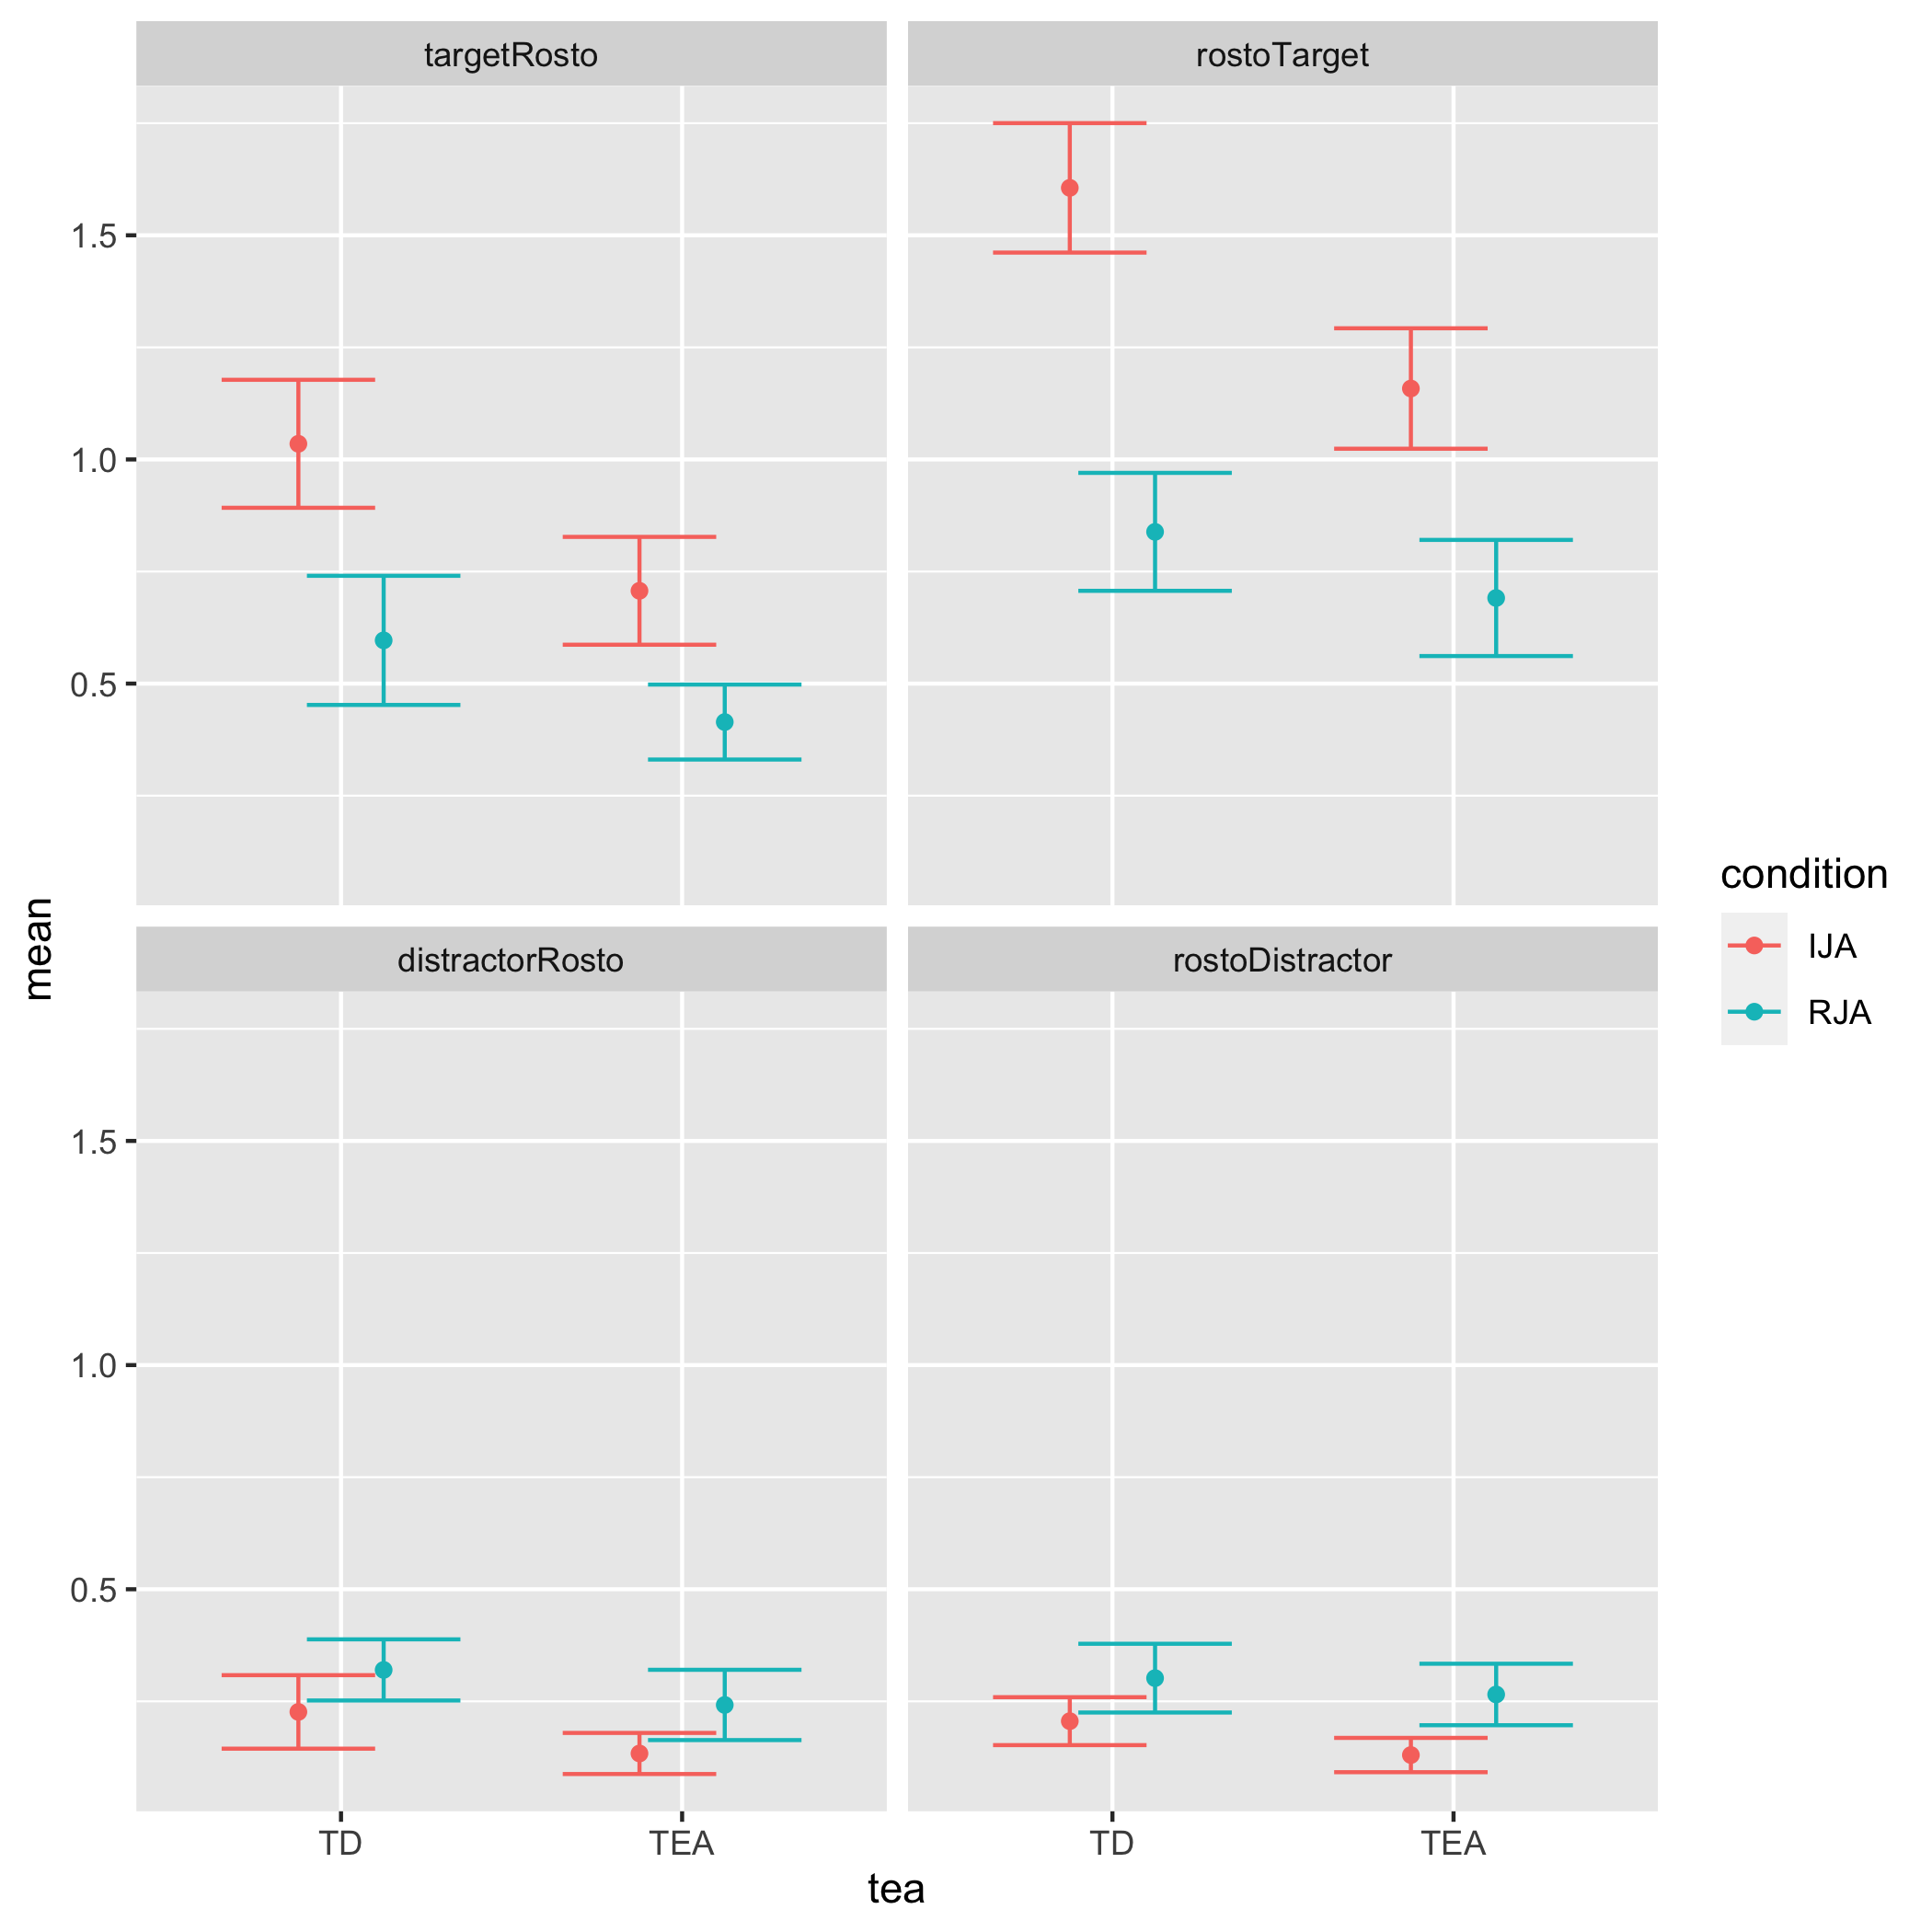
\includegraphics[scale=0.2]{./conditionVariableTeaAlternancia.png}}
  \centering
\end{figure}

\begin{figure}[H]
  \caption{Visualizing interaction between tea and variable. *Non significant}
  \noindent\makebox[\textwidth]{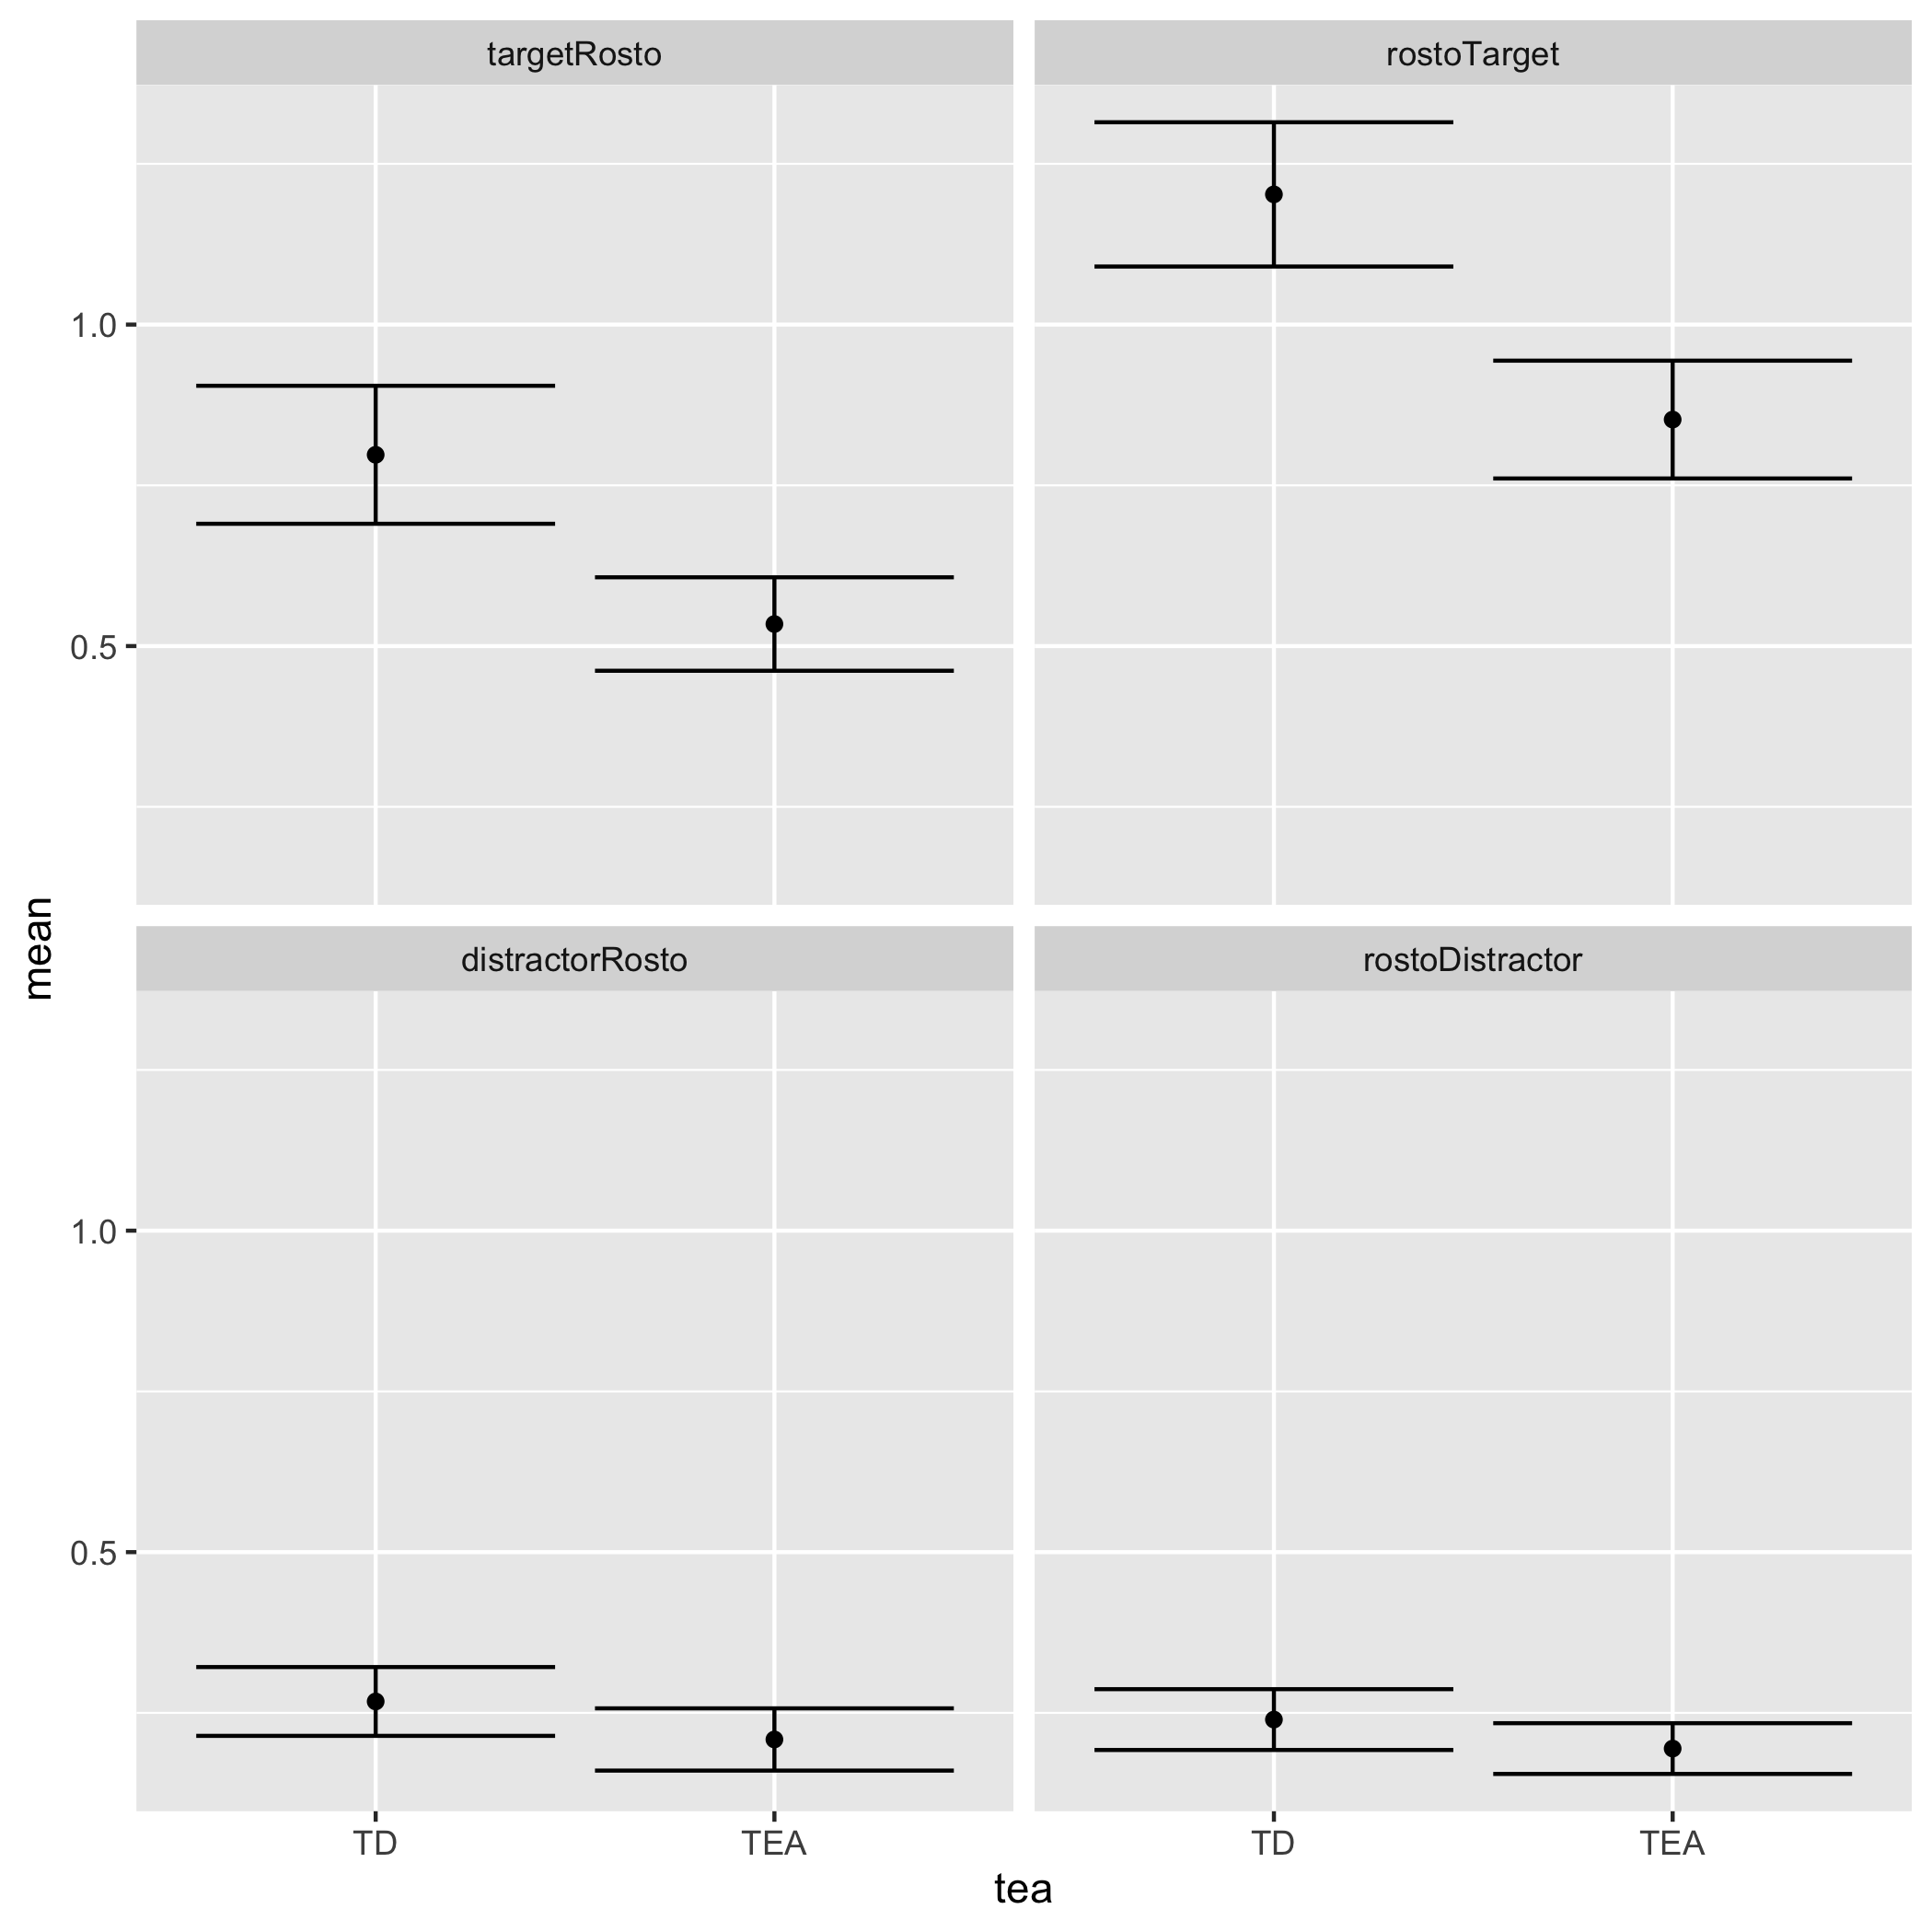
\includegraphics[scale=0.2]{./teaVariableAlternancia.png}}
  \centering
\end{figure}

\subsection{Proportion fixation}

%variable, condition*variable, tea*variable

\begin{figure}[H]
  \caption{Anova table for proportion fixation}
  \noindent\makebox[\textwidth]{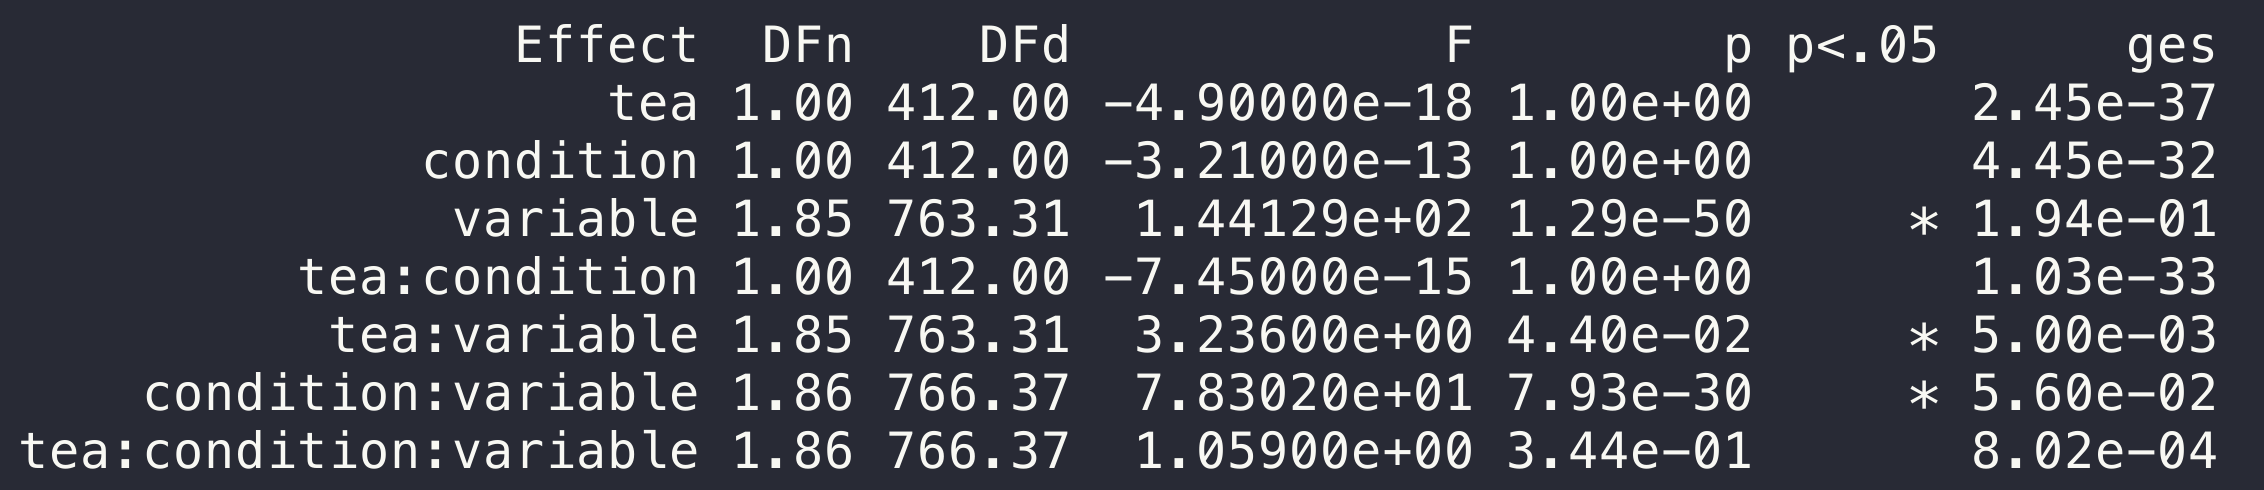
\includegraphics[scale=0.5]{./anovaProportions.png}}
  \centering
\end{figure}

\begin{figure}[H]
  \caption{Visualizing interaction of tea and variable}
  \noindent\makebox[\textwidth]{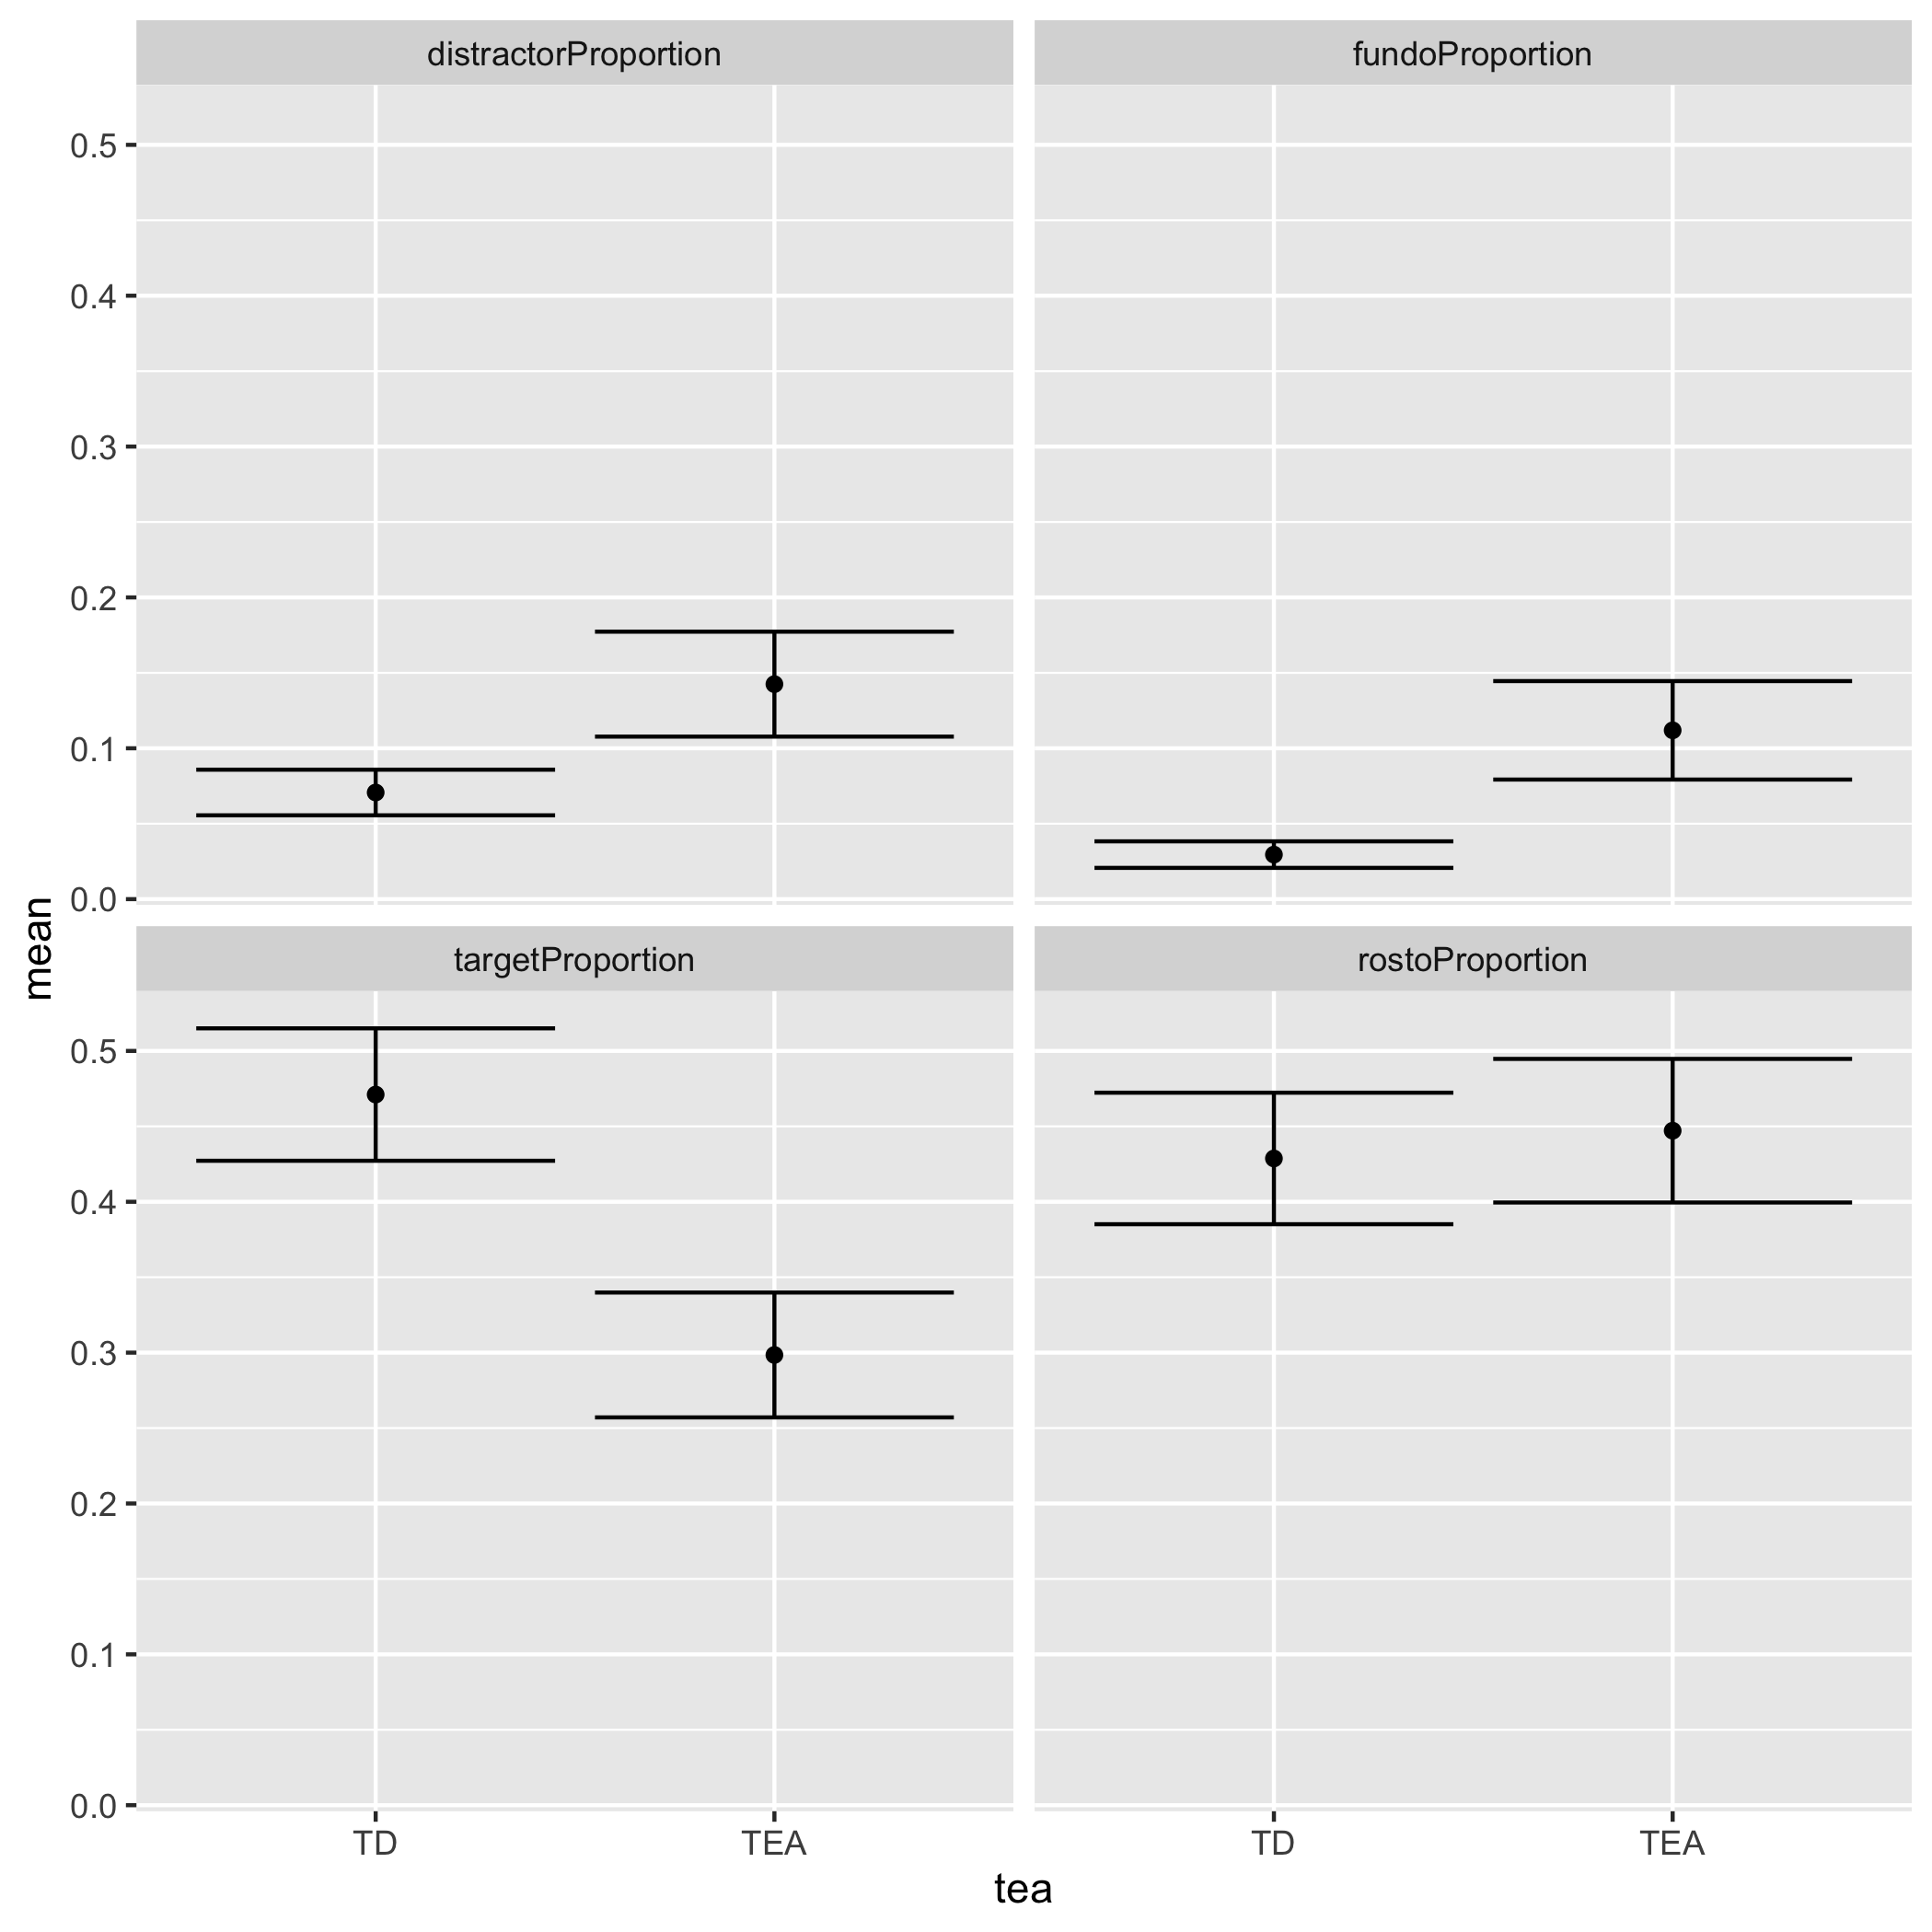
\includegraphics[scale=0.2]{./teaVariableProportion.png}}
  \centering
\end{figure}

\begin{figure}[H]
  \caption{Visualizing main effect of variable}
  \noindent\makebox[\textwidth]{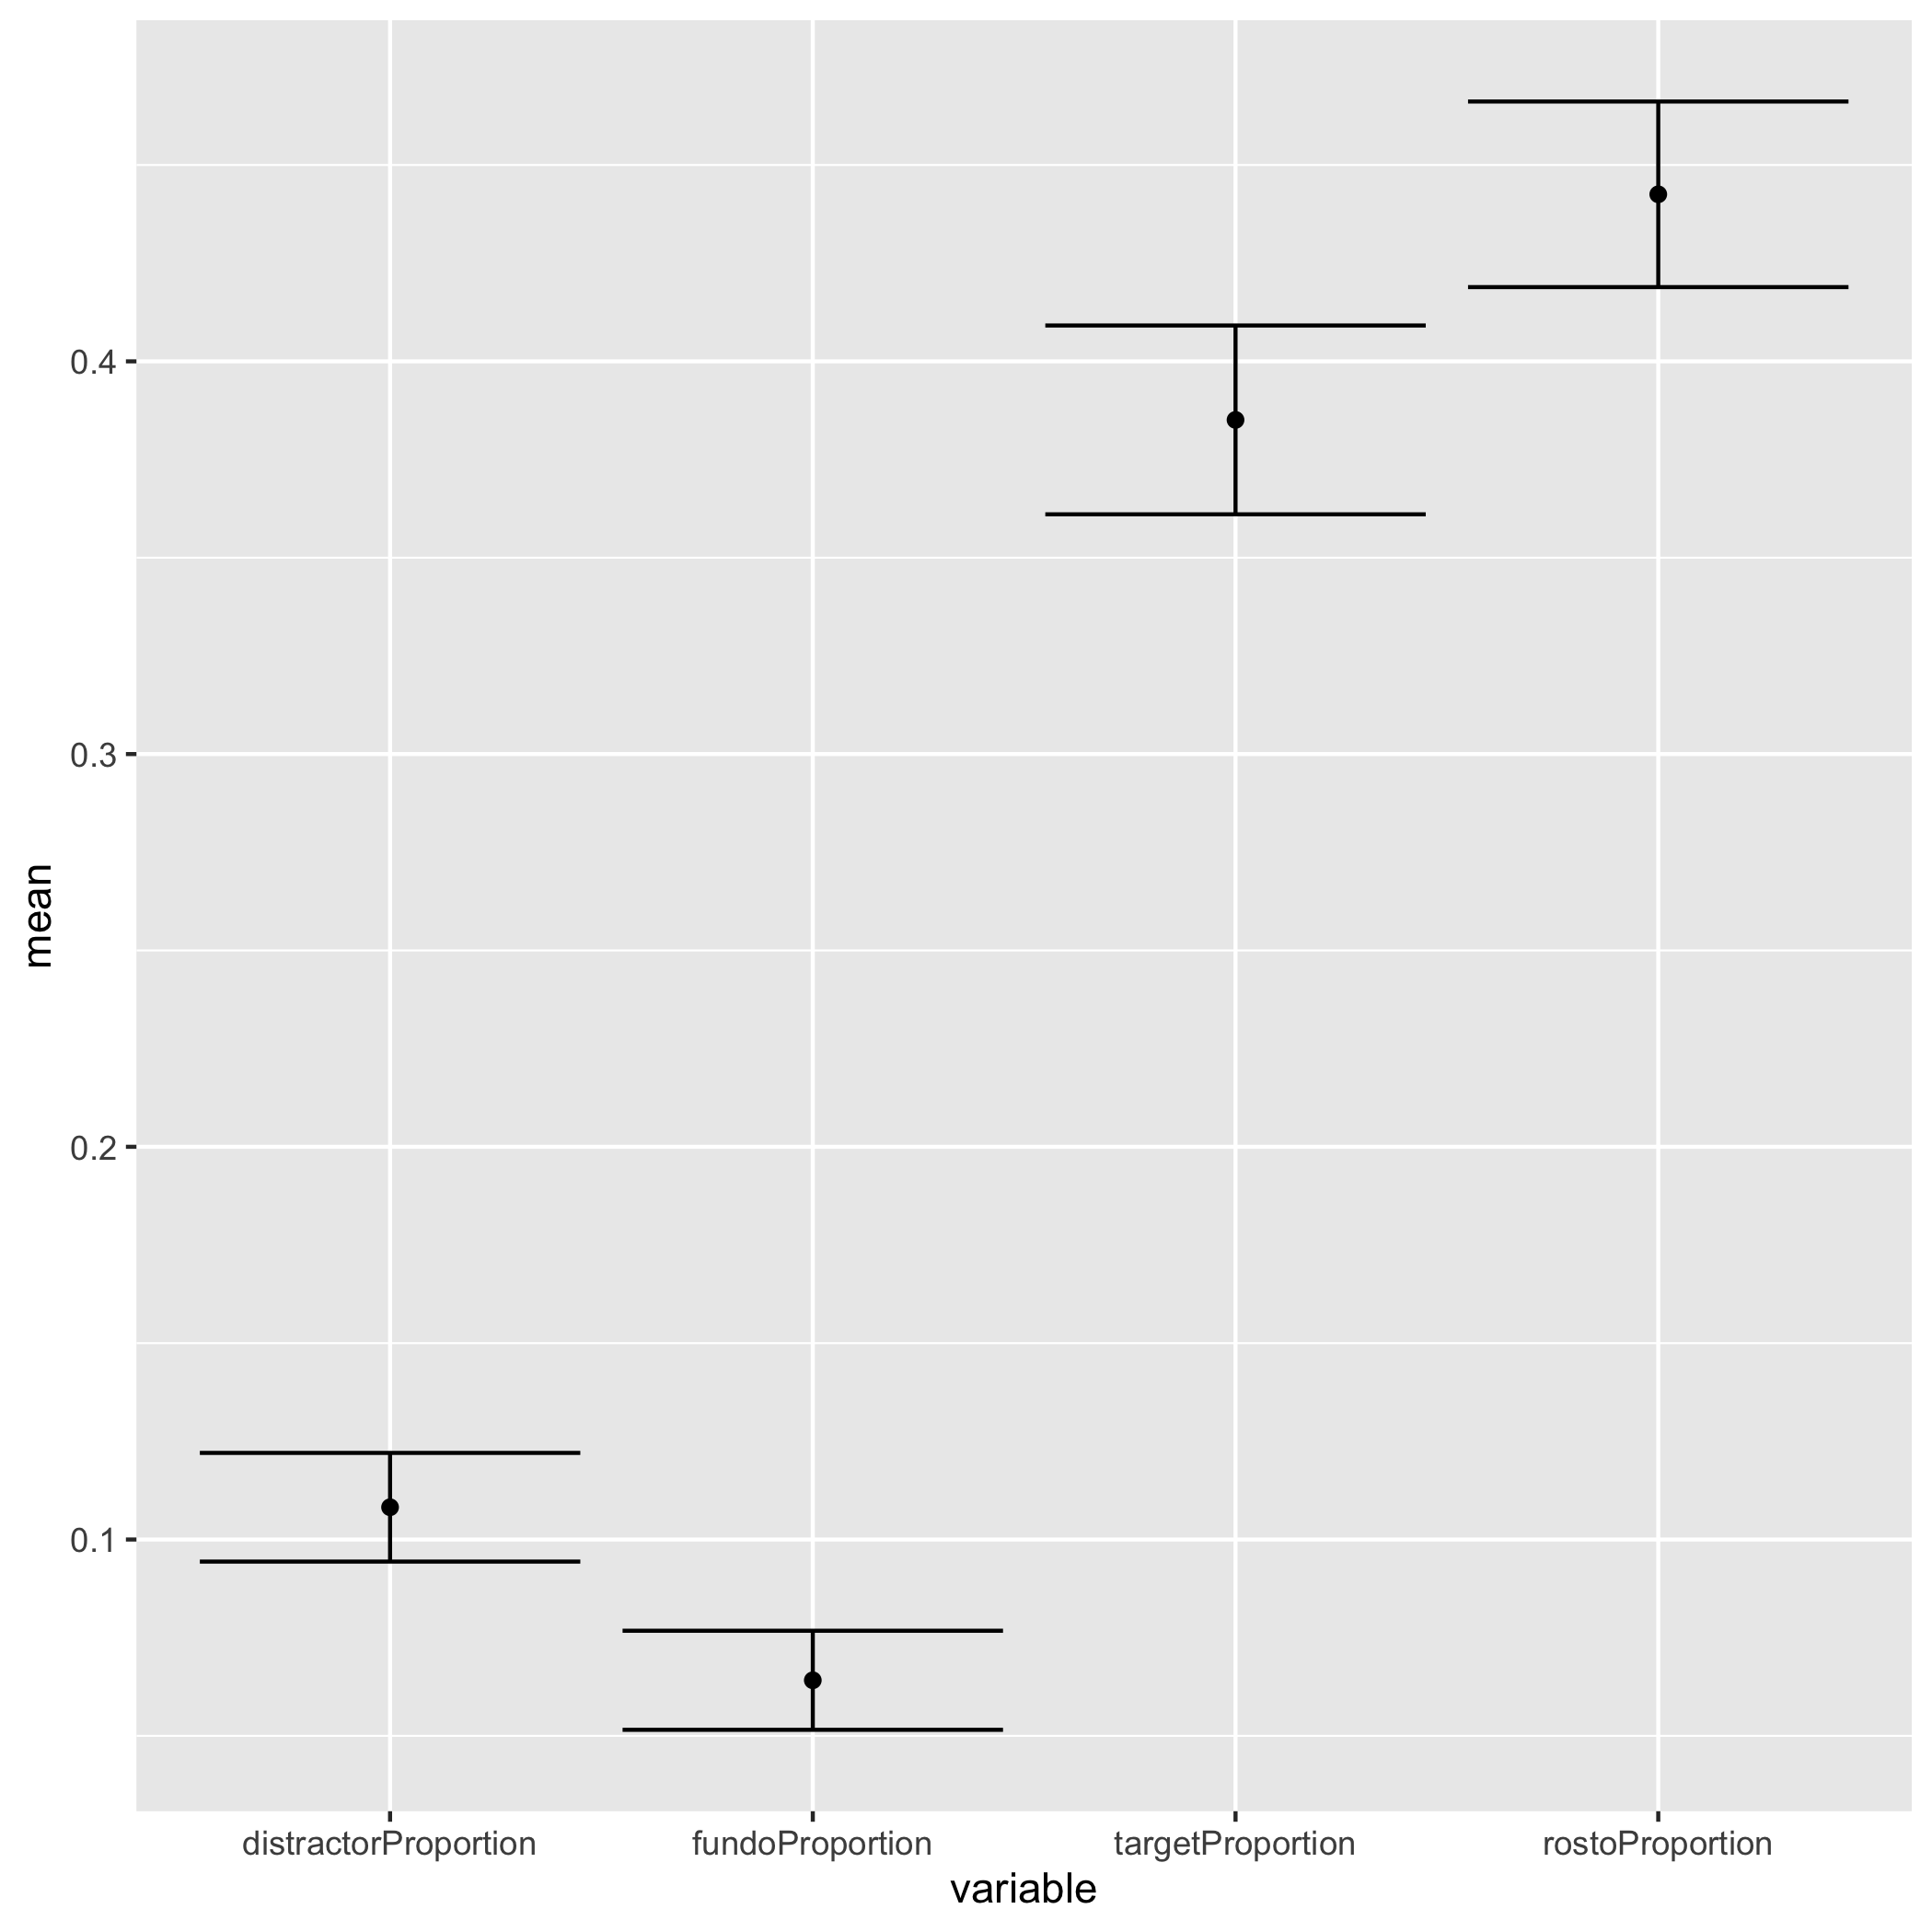
\includegraphics[scale=0.2]{./variableProportion.png}}
  \centering
\end{figure}

\begin{figure}[H]
  \caption{Visualizing interaction of condition and variable}
  \noindent\makebox[\textwidth]{\includegraphics[scale=0.2]{./condidionVariableProportion.png}}
  \centering
\end{figure}

Ho, D., Imai, K., King, G., \& Stuart, E. A. (2011). MatchIt: Nonparametric Preprocessing for Parametric Causal Inference. Journal of Statistical Software, 42(8), 1–28. https://doi.org/10.18637/jss.v042.i08

\end{document}
